\documentclass{article}
\usepackage{graphicx}
\begin{document}

\title{CS 3841 Lab 5: Let's Chat}
\author{Jeff Stubler \& Matt Edwards}
\date{24 October 2011}
\maketitle

\section*{Introduction}
We started this lab by discussing how we would design and implement it based on the given requirements. It was determined that new threads would be created to handle the UI, keyboard, time ticking, sending messages, receiving messages, and a controller thread to handle all of these. We split the work so Jeff would spend most of his time on the keyboard, time ticking, and sending and receiving of messages, while Matt would work primarily on the UI thread.

\section*{Things that went right and wrong}
Overall, this lab went well. In particular, two parts of this lab went well - the server and the UI implementation. Although the server took a considerable amount of time, the final result turned out quite well. Aside from the time commitment, nothing there was nothing that was too problematic in this lab. That being said, it did take some trial and error to create a UI with the desired panels and windows.

\section*{What we learned}
From this lab, we learned that programming sockets in C is a lot more difficult than programming sockets in Java, and protocols that are easy to use with Telnet are easier to develop. Also, we learned how to incorporate the ncurses library to create an elementary GUI with C.

\section*{Time Analysis}
In total Jeff spent about 15 hours working on this and Matt spent about 10. Most of Jeff's time was spent on the server and Matt's was divided among learning how to use ncurses and implementing the UI.

\section*{Chatd screenshots}
Figures~\ref{chatd-send} and \ref{chatd-receive} show telnet sessions with the chat server, sending and receiving messages or only sending, respectively. Using telnet, the headers given with
the different message types can be seen that are normally hidden by the UI for the chat system.

\begin{figure}[!h]
\begin{center}
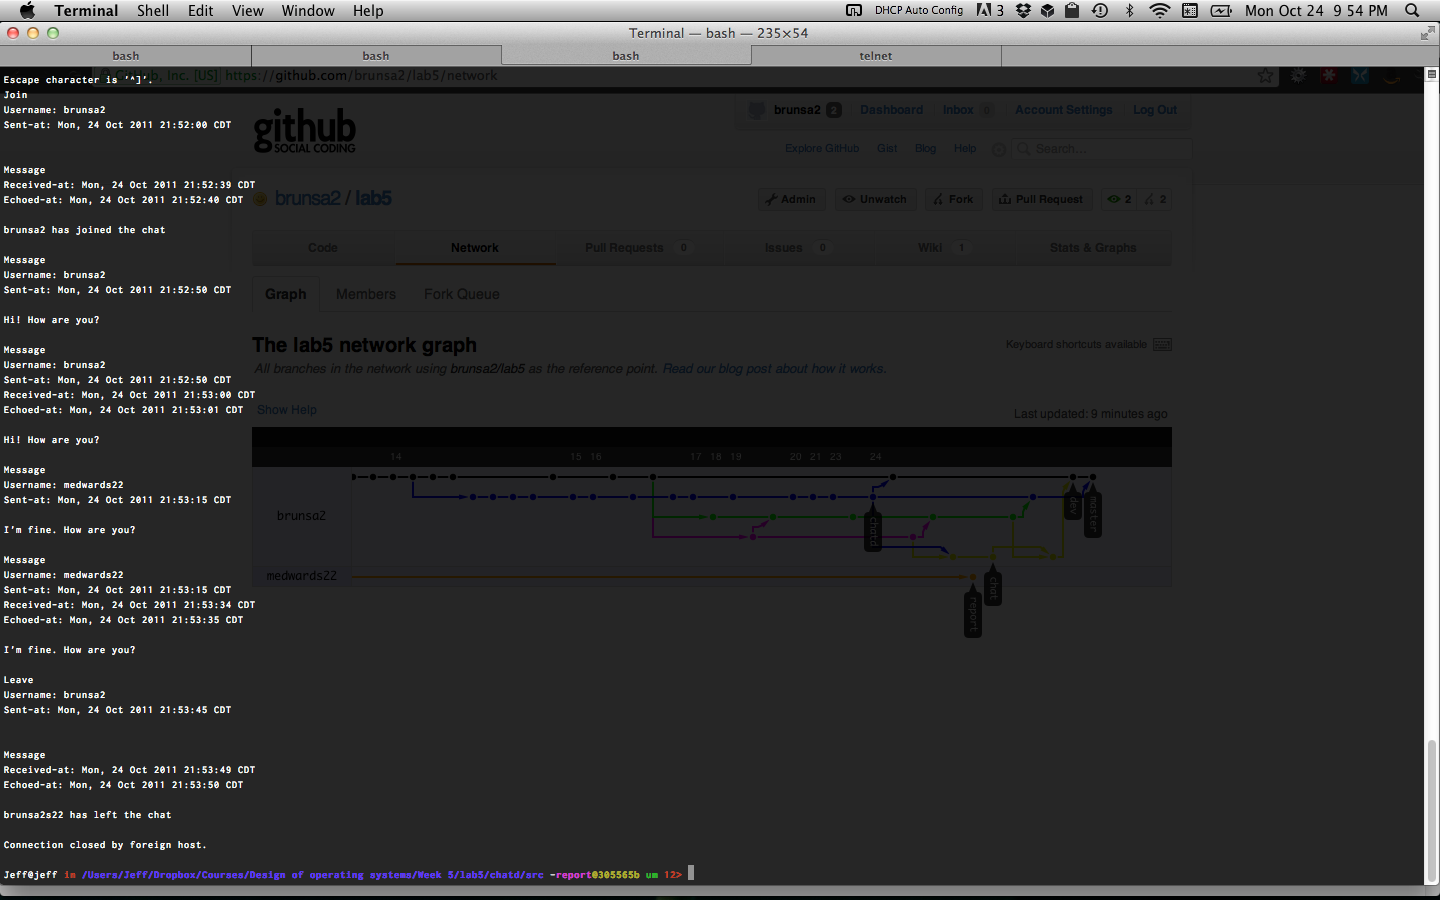
\includegraphics[scale=0.2]{send.png}
\end{center}
\caption{Telnet to chatd, sending and receiving}
\label{chatd-send}
\end{figure}

\begin{figure}[!h]
\begin{center}
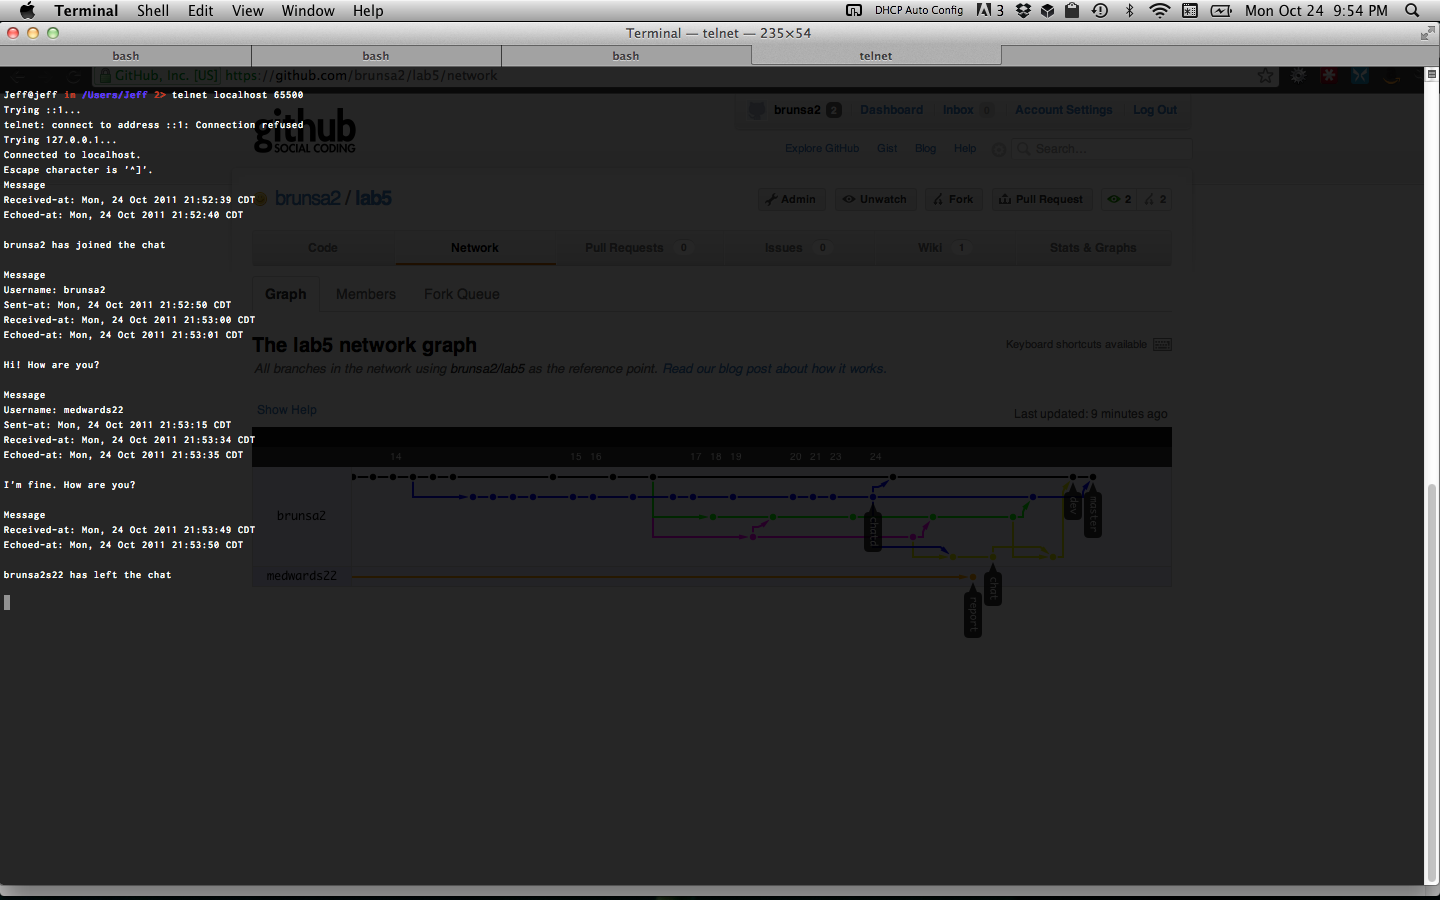
\includegraphics[scale=0.2]{receive.png}
\end{center}
\caption{Telnet to chatd, sending only}
\label{chatd-receive}
\end{figure}

\section*{Conclusion}
In this lab, we successfully constructed code using POSIX threads, protected against race conditions, communicated using sockets, and implemented a GUI with ncurses. We learned quite a bit from this lab and spent a decent amount of time making sure everything worked correctly.

\section*{Appendix: Source code}

\subsection*{controller.c}

\begin{verbatim}

/*
 * Jeff Stubler
 * CS 3841
 * Lab 5 -- UNIX chat program
 * 14 October 2011
 *
 * Main controller thread
 */

#include "controller.h"

void ctrl_thread(void) {
    int x = 0;
    for(x = 0; x < 5; x++) {
        sleep(10);
        printf("Alive\n");
    }
}

void clock_tick(void) {
    
}

void string_entered(void) {
    
}

void network_ready(void) {
    
}

void message_arrived(void) {
    
}

\end{verbatim}

\subsection*{controller.h}

\begin{verbatim}

/*
 * Jeff Stubler
 * CS 3841
 * Lab 5 -- UNIX chat program
 * 14 October 2011
 *
 * Main controller thread
 */

#ifndef CONTROLLER
#define CONTROLLER

#include <stdio.h>

#include "tick.h"
#include "keyboard.h"

void ctrl_thread(void);
void clock_tick(void);
void string_entered(void);
void network_ready(void);
void message_arrived(void);

#endif

\end{verbatim}

\subsection*{keyboard.c}

\begin{verbatim}

/*
 * Jeff Stubler
 * CS 3841
 * Lab 5 -- UNIX chat program
 * 13 October 2011
 *
 * Keyboard buffer system
 */

#include "keyboard.h"

#define KB_BUFFER_SIZE 16
#define KB_FIRST_TAIL 0
#define KB_FIRST_HEAD 1

#define adjusted_head(head) (head == 0 ? 16 : head)

//extern ncurses_initialized;
mutex_id kb_buffer_mutex = PTHREAD_MUTEX_INITIALIZER;

static char kb_buffer[KB_BUFFER_SIZE];
static int kb_buffer_head = KB_FIRST_HEAD, kb_buffer_tail = KB_FIRST_TAIL;

void *kb_thread(void *argument) {
    char next_character;
    //while(!ncurses_initialized);
    while(true) {
        next_character = getchar();
        lock(&kb_buffer_mutex);
        while(kb_buffer_head == kb_buffer_tail);
        kb_buffer[kb_buffer_head] = next_character;
        kb_buffer_head = (kb_buffer_head + 1) % KB_BUFFER_SIZE;
        unlock(&kb_buffer_mutex);
    }
    
    return NULL;
}

bool kb_has_key(void) {
    lock(&kb_buffer_mutex);
    if(adjusted_head(kb_buffer_head) - kb_buffer_tail == 1) {
        unlock(&kb_buffer_mutex);
        return false;
    } else {
        unlock(&kb_buffer_mutex);
        return true;
    }
}

char kb_get_key(void) {
    char next_key;
    lock(&kb_buffer_mutex);
    if(!kb_has_key()) {
        unlock(&kb_buffer_mutex);
        return '\0';
    } else {
        next_key = kb_buffer[kb_buffer_tail];
        kb_buffer_tail = (kb_buffer_head + 1) & KB_BUFFER_SIZE;
        unlock(&kb_buffer_mutex);
        return next_key;
    }
}

\end{verbatim}

\subsection*{keyboard.h}

\begin{verbatim}

/*
 * Jeff Stubler
 * CS 3841
 * Lab 5 -- UNIX chat program
 * 13 October 2011
 *
 * Keyboard buffer system
 */

#ifndef KEYBOARD
#define KEYBOARD

#include <stdio.h>
#include <stdbool.h>
#include <pthread.h>

#include "thread.h"

void *kb_thread(void *);
bool kb_has_key(void);
char kb_get_key(void);

#endif

\end{verbatim}

\subsection*{main.c}

\begin{verbatim}

/*
 * Jeff Stubler
 * CS 3841
 * Lab 5 -- UNIX chat program
 * 12 October 2011
 *
 * Main entry point for client, gathers arguments, starts threads, and acts as
 * main controller for system
 */

#include "main.h"

#define fatal_shutdown(message) fprintf(stderr, "%s\n", message); \
        exit(EXIT_FAILURE);

/* Variables for parsing command line arguments */
extern int optind, opterr, optopt;
extern char *optarg;
extern int network_error_code;

login_info login;

static void print_usage_and_exit_with_code(int exit_status) {
    fprintf(stderr, "Usage: chat [OPTION]... host\n"
            "Talk among other users connected to a chat server.\n\n"
            /*"-a\t\tJoin anonymously without greeting message\n"*/
            "-h, --help\tDisplay this help and exit\n"
            "-p\t\tSpecify port to connect to server on\n"
            "-u\t\tSet username to be displayed to chat members\n\n");
    exit(exit_status);
}

int main(int argc, char **argv) {
    int option, thread_error_code;
    thread_id kb_thread_id, tick_thread_id, ui_thread_id, network_thread_id;
    void *return_value;
    
    if(argc > 1 && strcmp(argv[1], "--help") == 0) {
        print_usage_and_exit_with_code(EXIT_SUCCESS);
    }
    
    while((option = getopt(argc, argv, ":ahp:u:")) != -1) {        
        switch(option) {
            case 'a':
                login.anonymous = true;
            case 'h':
                print_usage_and_exit_with_code(EXIT_SUCCESS);
            case 'p':
                if(login.port != NULL) {
                    free(login.port);
                }
                login.port = (char *) malloc(strlen(optarg));
                strcpy(login.port, optarg);
                break;
            case 'u':
                if(login.username != NULL) {
                    free(login.username);
                }
                login.username = (char *) malloc(strlen(optarg));
                strcpy(login.username, optarg);
                break;
            case ':':
                fprintf(stderr, "Missing argument for %c option\n\n", optopt);
                print_usage_and_exit_with_code(EXIT_FAILURE);
            case '?':
                fprintf(stderr, "Unrecognized flag %c\n\n", optopt);
                print_usage_and_exit_with_code(EXIT_FAILURE);
            default:
                fatal_shutdown("Unexpected response from option parser");
        }
    }
    
    if(optind < argc) {
        login.server = (char *) malloc(strlen(argv[optind]));
        strcpy(login.server, argv[optind]);
    } else {
        fprintf(stderr, "Missing host name\n\n");
        print_usage_and_exit_with_code(EXIT_FAILURE);
    }
    
    /* TODO: Check for null for any login block information and set it to a
     * default value */
    
    start_thread(&kb_thread_id, kb_thread, NULL);
    start_thread(&tick_thread_id, tick_thread, NULL);
    start_thread(&ui_thread_id, ui_thread, NULL);
    printf("Connecting...\n");
    start_thread(&network_thread_id, network_thread, NULL);
    
    sleep(2);
    if(network_error_code != 0) {
        printf("Could not connect\nError code %d\n", network_error_code);
        exit(EXIT_FAILURE);
    }
    
    ctrl_thread();
    
    free(login.username);
    free(login.server);
    free(login.port);
    
    return 0;
}

\end{verbatim}

\subsection*{network.c}

\begin{verbatim}

/*
 * Jeff Stubler
 * CS 3841
 * Lab 5 -- UNIX chat program
 * 14 October 2011
 *
 * Network startup thread
 */

#include "network.h"

extern login_info login;
int network_error_code;
int sock_fd;

void *network_thread(void *argument) {
    thread_id send_thread_id, receive_thread_id;
    struct addrinfo hints, *servinfo, *current_addr;
    int gai_error_code;
    
    memset(&hints, 0, sizeof(hints));
    hints.ai_family = AF_UNSPEC;
    hints.ai_socktype = SOCK_STREAM;
    
    if((gai_error_code = getaddrinfo(login.server, login.port, &hints, &servinfo)) != 0) {
        network_error_code = -1;
        return NULL;
    }
    
    for(current_addr = servinfo; current_addr != NULL; current_addr =       
            current_addr->ai_next) {
        if((sock_fd = socket(current_addr->ai_family,
                              current_addr->ai_socktype, current_addr->ai_protocol)) == -1) {
            continue;
        }
        
        if(connect(sock_fd, current_addr->ai_addr, current_addr->ai_addrlen) == -1) {
            close(sock_fd);
            continue;
        }
        
        break;
    }
    
    if(current_addr == NULL) {
        network_error_code = -1;
        return NULL;
    }
    
    freeaddrinfo(servinfo);
    
    network_ready();
    
    write(sock_fd,
          "Join\r\rUsername: brunsa2\r\n\r\n\r\n",
          strlen("Join\r\rUsername: brunsa2\r\n\r\n\r\n"));
    write(sock_fd,
          "Message\r\nUsername: brunsa2\r\n\r\nHi! How are you?\r\n\r\n",
          strlen("Message\r\nUsername: brunsa2\r\n\r\nHi! How are you?\r\n\r\n"));
    
    //start_joinable_thread(&send_thread_id, send_thread, &sock_fd);
    start_joinable_thread(&receive_thread_id, receive_thread, &sock_fd);
    
    join_thread(&send_thread_id);
    join_thread(&receive_thread_id);
    
    close(sock_fd);
    
    return NULL;
}

\end{verbatim}

\subsection*{network.h}

\begin{verbatim}

/*
 * Jeff Stubler
 * CS 3841
 * Lab 5 -- UNIX chat program
 * 14 October 2011
 *
 * Network startup thread
 */

#ifndef NETWORK
#define NETWORK

#include <stdio.h>
#include <syslog.h>
#include <stdbool.h>
#include <stdlib.h>
#include <unistd.h>
#include <string.h>
#include <errno.h>
#include <sys/types.h>
#include <sys/socket.h>
#include <netinet/in.h>
#include <netdb.h>
#include <arpa/inet.h>
#include <sys/wait.h>

#include "thread.h"
#include "main.h"

typedef struct {
    char *username;
    char *message_text;
} message;

#include "send.h"
#include "receive.h"

void *network_thread(void *);

#endif

\end{verbatim}

\subsection*{receive.c}

\begin{verbatim}

/*
 * Jeff Stubler
 * CS 3841
 * Lab 5 -- UNIX chat program
 * 14 October 2011
 *
 * Network receive thread
 */

#include "receive.h"

void *receive_thread(void *argument) {
    return NULL;
}

message *get_message(void) {
    return NULL;
}

\end{verbatim}

\subsection*{receive.h}

\begin{verbatim}

/*
 * Jeff Stubler
 * CS 3841
 * Lab 5 -- UNIX chat program
 * 14 October 2011
 *
 * Network receive thread
 */

#ifndef NETWORK_RECEIVE
#define NETWORK_RECEIVE

#include <stdlib.h>

#include "network.h"

void *receive_thread(void *);
message *get_message(void);

#endif

\end{verbatim}

\subsection*{send.c}

\begin{verbatim}

/*
 * Jeff Stubler
 * CS 3841
 * Lab 5 -- UNIX chat program
 * 14 October 2011
 *
 * Network send thread
 */

#include "send.h"

void *send_thread(void *argument) {
    int sock_fd = (int) ((void *) argument);
    
    write(sock_fd,
          "Join\r\rUsername: brunsa2\r\n\r\n\r\n",
          strlen("Join\r\rUsername: brunsa2\r\n\r\n\r\n"));
    write(sock_fd,
          "Message\r\nUsername: brunsa2\r\n\r\nHi! How are you?\r\n\r\n",
          strlen("Message\r\nUsername: brunsa2\r\n\r\nHi! How are you?\r\n\r\n"));
    
    return NULL;
}

void send_message(message *sending_message) {
    
}

\end{verbatim}

\subsection*{send.h}

\begin{verbatim}

/*
 * Jeff Stubler
 * CS 3841
 * Lab 5 -- UNIX chat program
 * 14 October 2011
 *
 * Network send thread
 */

#ifndef NETWORK_SEND
#define NETWORK_SEND

#include <stdlib.h>

#include "network.h"

void *send_thread(void *);
void send_message(message *);

#endif

\end{verbatim}

\subsection*{thread.c}

\begin{verbatim}

/*
 * Jeff Stubler
 * CS 3841
 * Lab 5 -- UNIX chat program
 * 12 October 2011
 *
 * Thread convenience functions, wraps around Pthreads
 */

#include "thread.h"

#define fatal_shutdown(message) fprintf(stderr, "%s\n", message); \
exit(EXIT_FAILURE);

/* TODO: Look further at thread priority */

void start_thread(pthread_t *thread, void *(* thread_function)(void *),
                  void *argument) {
    int thread_error_code;
    pthread_attr_t attributes;
    
    thread_error_code = pthread_attr_init(&attributes);
    if(thread_error_code != 0) {
        fatal_shutdown("Error initializing thread attributes");
    }
    
    thread_error_code = pthread_attr_setdetachstate(&attributes,
                                                    PTHREAD_CREATE_DETACHED);
    if(thread_error_code != 0) {
        fatal_shutdown("Error setting thread detach state attribute");
    }
    
    thread_error_code = pthread_create(thread, &attributes, thread_function,
                                       argument);
    if(thread_error_code != 0) {
        fatal_shutdown("Error starting thread");
    }
    
    thread_error_code = pthread_attr_destroy(&attributes);
    if(thread_error_code != 0) {
        fatal_shutdown("Error destroying attributes");
    }
}

void start_joinable_thread(pthread_t *thread, void *(* thread_function)(void *),
                           void *argument) {
    int thread_error_code;
    
    thread_error_code = pthread_create(thread, NULL, thread_function, argument);
    if(thread_error_code != 0) {
        fatal_shutdown("Error starting thread");
    }
}

void join_thread(pthread_t *thread) {
    pthread_t joined_thread;
    memcpy(&joined_thread, thread, sizeof(thread));
    pthread_join(joined_thread, NULL);
}

void initialize_mutex(mutex_id *mutex) {
    int mutex_error_code;
    mutex_error_code = pthread_mutex_init(mutex, NULL);
    if(mutex_error_code != 0) {
        fatal_shutdown("Error initializing mutex");
    }
}

void lock(mutex_id *mutex) {
    pthread_mutex_lock(mutex);
}

void unlock(mutex_id *mutex) {
    pthread_mutex_unlock(mutex);
}

void destroy_mutex(mutex_id *mutex) {
    int mutex_error_code;
    unlock(mutex);
    mutex_error_code = pthread_mutex_destroy(mutex);
    if(mutex_error_code != 0) {
        fatal_shutdown("Error destroying mutex");
    }
}

\end{verbatim}

\subsection*{thread.h}

\begin{verbatim}

/*
 * Jeff Stubler
 * CS 3841
 * Lab 5 -- UNIX chat program
 * 12 October 2011
 *
 * Thread convenience functions, wraps around Pthreads
 */

#ifndef THREADS
#define THREADS

#include <pthread.h>
#include <stdio.h>
#include <stdlib.h>
#include <string.h>

typedef pthread_t thread_id;
typedef pthread_mutex_t mutex_id;

void start_thread(pthread_t *, void *(* thread_function)(void *), void *);
void start_joinable_thread(pthread_t *, void *(* thread_function)(void *),
                           void *);
void join_thread(pthread_t *);
void initialize_mutex(mutex_id *);
void lock(mutex_id *);
void unlock(mutex_id *);
void destroy_mutex(mutex_id *);

#endif

\end{verbatim}

\subsection*{tick.c}

\begin{verbatim}

/*
 * Jeff Stubler
 * CS 3841
 * Lab 5 -- UNIX chat program
 * 14 October 2011
 *
 * Tick counting thread
 */

#include "tick.h"

#define MICROSECONDS_BETWEEN_CLOCK_UPDATE 1000000

static start_ticks, elapsed_ticks;

void *tick_thread(void *argument) {
    start_ticks = time(NULL);
    
    while(true) {
        elapsed_ticks = time(NULL) - start_ticks;
        usleep(MICROSECONDS_BETWEEN_CLOCK_UPDATE);
        clock_tick();
    }
    
    return NULL;
}

int get_elapsed_ticks(void) {
    return elapsed_ticks;
}

\end{verbatim}

\subsection*{tick.h}

\begin{verbatim}

/*
 * Jeff Stubler
 * CS 3841
 * Lab 5 -- UNIX chat program
 * 14 October 2011
 *
 * Tick counting thread
 */

#ifndef TICK
#define TICK

#include <stdio.h>
#include <time.h>
#include <stdbool.h>

#include "controller.h"

void *tick_thread(void *);
int get_elapsed_ticks(void);

#endif

\end{verbatim}

\subsection*{daemon.c}

\begin{verbatim}



\end{verbatim}

\subsection*{daemon.h}

\begin{verbatim}



\end{verbatim}

\subsection*{main.c}

\begin{verbatim}



\end{verbatim}

\end{document}
